% Chapter 10

\chapter{Diseño de Software y Hardware} % Write in your own chapter title
\label{Chapter10}
\lhead{Capítulo 10. \emph{Diseño}} % Write in your own chapter title to set the page header

La investigación basada en el estado del arte Capítulo \ref{Chapter6}, determinó que la estructura que mejor se acopla al tipo de problema es una ANN de tres capas, tres neuronas en la capa de entrada para analizar las variables de Flujo, Precipitación y Humedad Relativa, una capa oculta con mínimo tres neuronas y finalmente una neurona en la capa de salida. Por otra parte, también determinó que es necesario escalar el sistema de detección proporcionalmente según la necesidad de resolución en la medición, esto es necesario cuando se desea determinar con mayor precisión el riesgo de inundación del área examinada.

%Dado el problema, según el estado del arte, la mejor estructura de análisis es una Red Neuronal Artificial que pueda recibir al menos 3 datos (Flujo, Precipitación y Humedad Relativa) por nodo de medición. Esta medición debe ser instantánea y dependiendo de las condiciones meteorológicas; es decir, si la probabilidad de una inundación incrementa analizar los datos de los múltiples nodos que componen el ecosistema de monitoreo del río a una frecuencia mas alta, de forma concurrente y poder responder a tiempo ante una emergencia alertando al centro de control local. 

%tek Revisar redacción...

\section{Diseño de Hardware}

Diseñar el hardware implica tener en cuenta las diferentes etapas del desarrollo del mismo; en este caso, es necesario conocer cómo funcionan el sintetizador de alto nivel Vivado HLS y el sintetizador de hardware Vivado Design Suite. Se estableció una metodología que permite establecer el mejor diseño de hardware: en primera instancia se debe realizar un análisis de cuáles son las posibles optimizaciones que puedan reducir la latencia total del circuito una vez sintetizado y cuáles podrían incrementarla.

\begin{enumerate}
\item Desarrollar la ANN usando lenguage C++.
\item Sintetizar el hardware usando Vivado HLS.
\item Analizar latencia y uso de recursos obtenidos en el reporte de síntesis.
\item Aplicar optimizaciones de hardware.
\item Repetir desde 2 hasta obtener el mínimo entre latencia y uso de recursos.
\end{enumerate}

Para este circuito se determinó que la latencia mínima se podría obtener usando las siguientes optimizaciones luego de analizar el código de la ANN, los bloques de memoria requeridos para realizar los bursts de memoria que provee la interfaz AXI, la cantidad de bucles y la cantidad de tareas que se realizan al interior del hardware.

\begin{enumerate}
\item Dataflow: Aplicable a tareas
\item Pipeline: Aplicable a bucles
\item Unroll: Aplicable a bucles
\end{enumerate}

\subsection{Diseño de la Red Neuronal Artificial}

Como se mencionó en el Capítulo \ref{Chapter7}, las redes neuronales son sistemas concurrentes capaces de aprender y realizar tareas para las que han sido entrenadas; por ejemplo, detección de patrones, clasificación, implementación de modelos matemáticos y fusión de datos. Por esta razón, es que se decide aplicarla a este problema, pues se desconoce la interacción entre las variables meteorológicas y físicas que afectan el nivel de los ríos provocando una inundación.

La Red Neuronal Artificial a implementar debe componerse de una capa de entrada con tres neuronas, un mínimo de tres neuronas en la capa oculta de la red y finalmente una neurona de salida, todo esto por nodo de medición en campo. Así pues, si se requieren analizar los datos provenientes de múltiples fuentes, se deberán instanciar tantas Redes Neuronales como nodos disponibles se tengan. La figura \ref{fig:networkDesign} muestra el diseño de la red implementada, en ella se puede observar el diseño básico, cada nodo de sensores se compone de una tripleta de neuronas a la entrada y en la capa oculta para ser por una neurona en la capa de salida la cual es la encargada de entregar el resultado de la estimación.

%La implementación de la red neuronal se compone de múltiples entradas totalmente conectadas entre sí; para el caso básico de muestreo se requieren como mínimo tres entradas y tres neuronas en la capa oculta. Para el caso en que se requieran analizar múltiples sensores, se deberían adicionar entradas tantos sensores se tengan disponibles y una capa oculta con igual número de neuronas como nodos de entrada a la red, véase la Figura \ref{fig:networkDesign}.

%tek Revisar redacción

\begin{figure}[H]
\centering
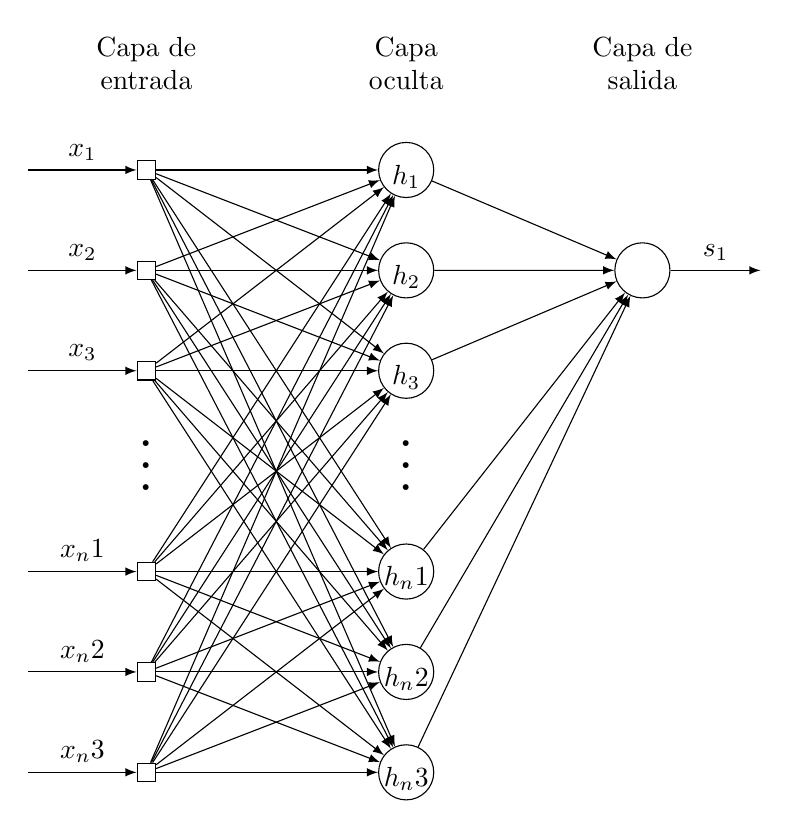
\begin{tikzpicture}[x=1.5cm, y=1.5cm,
every neuron/.style={ 
    circle,
    draw,
    minimum size=0.7cm
  },
every input/.style={
    draw,
  },
every layer/.style={
    draw=none, 
    scale=2,
    execute at begin node=\color{black}$\ldots$
  },
neuron missing/.style={
    draw=none, 
    scale=2,
    text height=0.25cm,
    execute at begin node=\color{black}$\vdots$
  }
]
\foreach \m/\l [count=\y] in {1,2,3,missing,4,5,6}
  \node [every input/.try, neuron \m/.try] (input-\m) at (-0.7,2.5-\y*0.85) {};

\foreach \m [count=\y] in {1,2,3,missing,4,5,6}
  \node [every neuron/.try, neuron \m/.try ] (hidden1-\m) at (1.5,2.5-\y*0.85) {};

% \foreach \m [count=\y] in {1,2,3,4}
%   \node [every layer/.try] (empty-\m) at (2.5,2.5-\y*0.8) {};
  
%   \foreach \m [count=\y] in {1,2,missing,3}
%   \node [every neuron/.try, neuron \m/.try ] (hidden2-\m) at (3.5,2.5-\y*0.85) {};
 
\foreach \m [count=\y] in {1}%,2,missing,3}
  \node [every neuron/.try, neuron \m/.try ] (output-\m) at (3.5,2.5-\y*1.7) {};

\foreach \l [count=\i] in {1,2,3,n1,n2,n3}
  \draw [latex-] (input-\i) -- ++(-1,0)
    node [above, midway] {$x_\l$};

\foreach \l [count=\i] in {1,2,3,n1,n2,n3}
  \node [above] at (hidden1-\i.south) {$h_\l$}; 

\foreach \l [count=\i] in {1}%,2,n}
  \draw [-latex] (output-\i) -- ++(1,0)
    node [above, midway] {$s_\l$};
  
\foreach \i in {1,...,6}
  \foreach \j in {1,...,6}
    \draw [-latex] (input-\i) -- (hidden1-\j);

\foreach \i in {1,...,6}
  \foreach \j in {1,...,1}
    \draw [-latex] (hidden1-\i) -- (output-\j);

\node [align=center, above] at (-0.7,2.25) {Capa de \\ entrada};
\node [align=center, above] at (1.5,2.25) {Capa \\ oculta};
\node [align=center, above] at (3.5,2.25) {Capa de \\ salida};
%\draw [decorate,decoration={brace,amplitude=10pt}] (1.2,2) -- (3.8,2);
\end{tikzpicture}
\caption{Diseño de la red neuronal}
\label{fig:networkDesign}
\end{figure}
 
\subsection{Función de salida de la red neuronal}

Uno de los parámetros que más influye en la veracidad de la estimación de una red neuronal es la función de activación de las neuronas, ver Tabla \ref{tab:funactivacion}. Según el estado del arte, la función de activación más común para este tipo de problemas es la función tangente sigmoidal \citep{floodfc1}, representada en la Ecuación \ref{eq:tansig} y la Figura \ref{fig:tansig}.

\begin{equation}\label{eq:tansig}
\varphi(u) = \dfrac{2}{1+e^{-2u}}-1
\end{equation}

\begin{figure}[H]
\centering
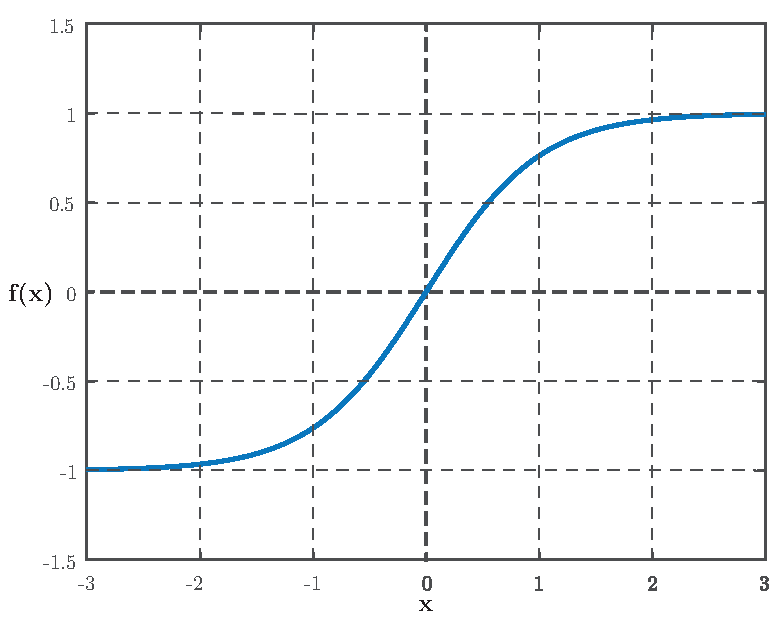
\includegraphics[scale=0.8]{./Figures/TANSIG.pdf}
\caption[Red neuronal en árbol]{Tangente sigmoidal}
\label{fig:tansig}
\end{figure}

La Ecuación \ref{eq:tansig} muestra que, para calcular la función tangente sigmoidal, es necesario realizar cómputos de complejos como los exponenciales que se pueden ver altamente afectados por el error que pueda introducir la unidad que los pueda calcular. Por otra parte, implementar este tipo de cálculos directamente sobre el hardware de la FPGA sería altamente costoso en términos de recursos y latencia por el simple hecho de utilizar punto flotante. Para resolver el problema se optó por realizar una implementación donde se discretiza la función continua, de tal forma que el bus de direcciones alcance máximo 12bits, es decir 4096 posiciones de memoria (se eligen 12b debido a que el sintetizador presenta problemas si se elige un bus de direcciones más grande al mapear una memoria ROM).

\subsection{Código fuente Red Neuronal Artificial}

A continuación se muestra de forma simplificada el diseño de la ANN en código fuente usando el lenguaje de programación C++

\begin{verbatim}
TOPANN ( fix *Inputs, fix *Outputs, fix *layerWeight, fix *layerBias,
  fix *outputLayerWeight, fix *outputLayerBias )
{  
  // Creación de buffers de memoria
  fix BurstInputs[DATASET_INPUTS];// Buffer local que garantiza el Burst
  fix layerResult[NEURONS];       // Permite reciclar el HW de las capas

  memcpy ( BurstInputs, (const fix *) Inputs,
    DATASET_INPUTS * sizeof(fix) );  // Mecanismo que activa el Burst
  
  // Ejecución del algoritmo de la ANN
  ANN ( BurstInputs, BurstOutputs, layerResult, Weights, ... )
  
  // Burst de salida
  memcpy ( (fix *) Outputs, layerResult, sizeof (fix) * OUTPUTS );
}
\end{verbatim}

Como se observa en el código anterior, la única diferencia entre una red de $3$ entradas y una de $N$ entradas son las definiciones de \texttt{DATASET\_INPUTS} y \texttt{NEURONS}, que definen respectivamente, cuántas entradas va a tener la red y la cantidad de neuronas en la capa oculta. Es por esto que se hace necesario sintetizar la cantidad de circuitos como variaciones de estas configuraciones.

\subsection{Puertos de entrada y salida AXI}

Dado que se requieren manipular grandes cantidades de datos provenientes de la red de sensores, se hace necesario que la ANN cuente con la instrumentación necesaria. En este caso, se optó por usar el máximo ancho de banda posible disponible en la arquitectura ZYNQ 7000; este es otorgado por el bus AMBA. Para lograr el máximo ancho de banda se requiere que el hardware realice un llamado en bloque a la memoria partiendo de una dirección base otorgada como dependencia en la entidad más alta como un apuntador (\texttt{* Inputs} y \texttt{* Outputs}) y realizar un llamado a la función \texttt{memcpy}, la cual activa el pipelining y las optimizaciones del bus en tiempo de síntesis; este proceso se conoce como MEMORY BURST TRANSACTION, véase la Figura \ref{fig:memBurst}.

\begin{figure}[H]
	\centering
		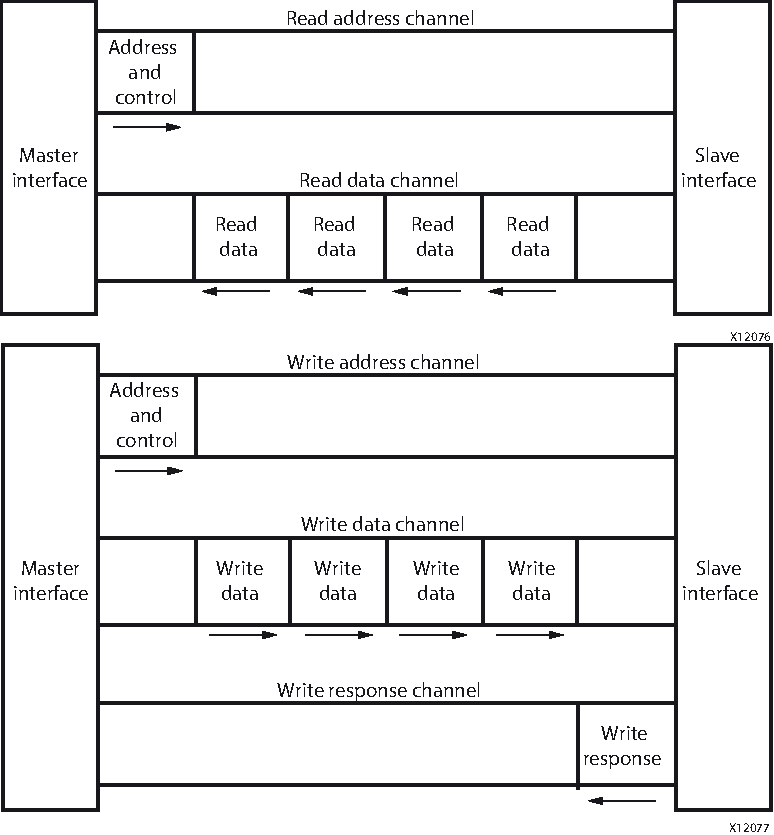
\includegraphics[scale=0.8]{./Figures/I2.pdf}
	\caption{Memory burst transaction \citep{AXI2017}}
	\label{fig:memBurst}
\end{figure}

Finalmente, es necesario determinar qué tipo de datos se usarán para realizar las operaciones a nivel de los datos. En este caso, para garantizar una baja latencia y un bajo uso de recursos, se optó por un ancho del bus de 32b definido en código como \texttt{fix}, el cual es una definición de 32b con 8b para la parte entera y 24b para la parte decimal, la cual puede ser ajustada de acuerdo a la necesidad.

\subsection{Optimizaciones de Hardware}

En la sub sección anterior se definió el diseño general de la ANN sin optimizaciones de hardware más allá de las dadas por la interfaz AXI. En esta sub sección se adicionarán las optmizaciones y los criterios de diseño para dejar una u otra optimización.

Previo a la síntesis, es necesario determinar cuáles son las optimizaciones adecuadas para el tipo de problema: del espectro de opciones, es necesario conocer bien el manual del Vivado HLS y las condiciones que deben cumplirse para aplicar las directivas, pues su disposición puede ser tanto positiva como negativa dependiendo de cómo se implementen. Tras analizar el código fuente, se estableció que, debido a la dependencia de los datos entre capas, el circuito se ve altamente beneficiado por mecanismos como el pipeline y el paralelismo de las diferentes tareas que se realizan. Una vez aplicadas las optimizaciones, es necesario analizar el reporte de síntesis y establecer si existen problemas con el ancho de banda de la memoria, el cual es un problema típico de este tipo de circuitos, en los que, debido a la alta concurrencia, el acceso a la RAM se ve afectado, teniendo que arbitrarse el acceso, aumentando en consecuencia de manera drástica la latencia total del circuito.

La Figura \ref{fig:latIntFloat} muestra la latencia e intervalo de datos para las diferentes optimizaciones. Estas están definidas en clocks y cada una brinda información importante para la implementación final; el intervalo indica cada cuántos clocks es posible introducir un nuevo dato al circuito para que pueda ser procesado y la latencia indica cuánto tarda un dato para ser procesado. En este caso, la combinación de las directivas DATAFLOW y PIPELINE permite obtener el menor intervalo en punto flotante, pero se ve superado por PIPELINE puro en cuanto a reducción de la latencia.

\begin{figure}[!ht]
	\centering
		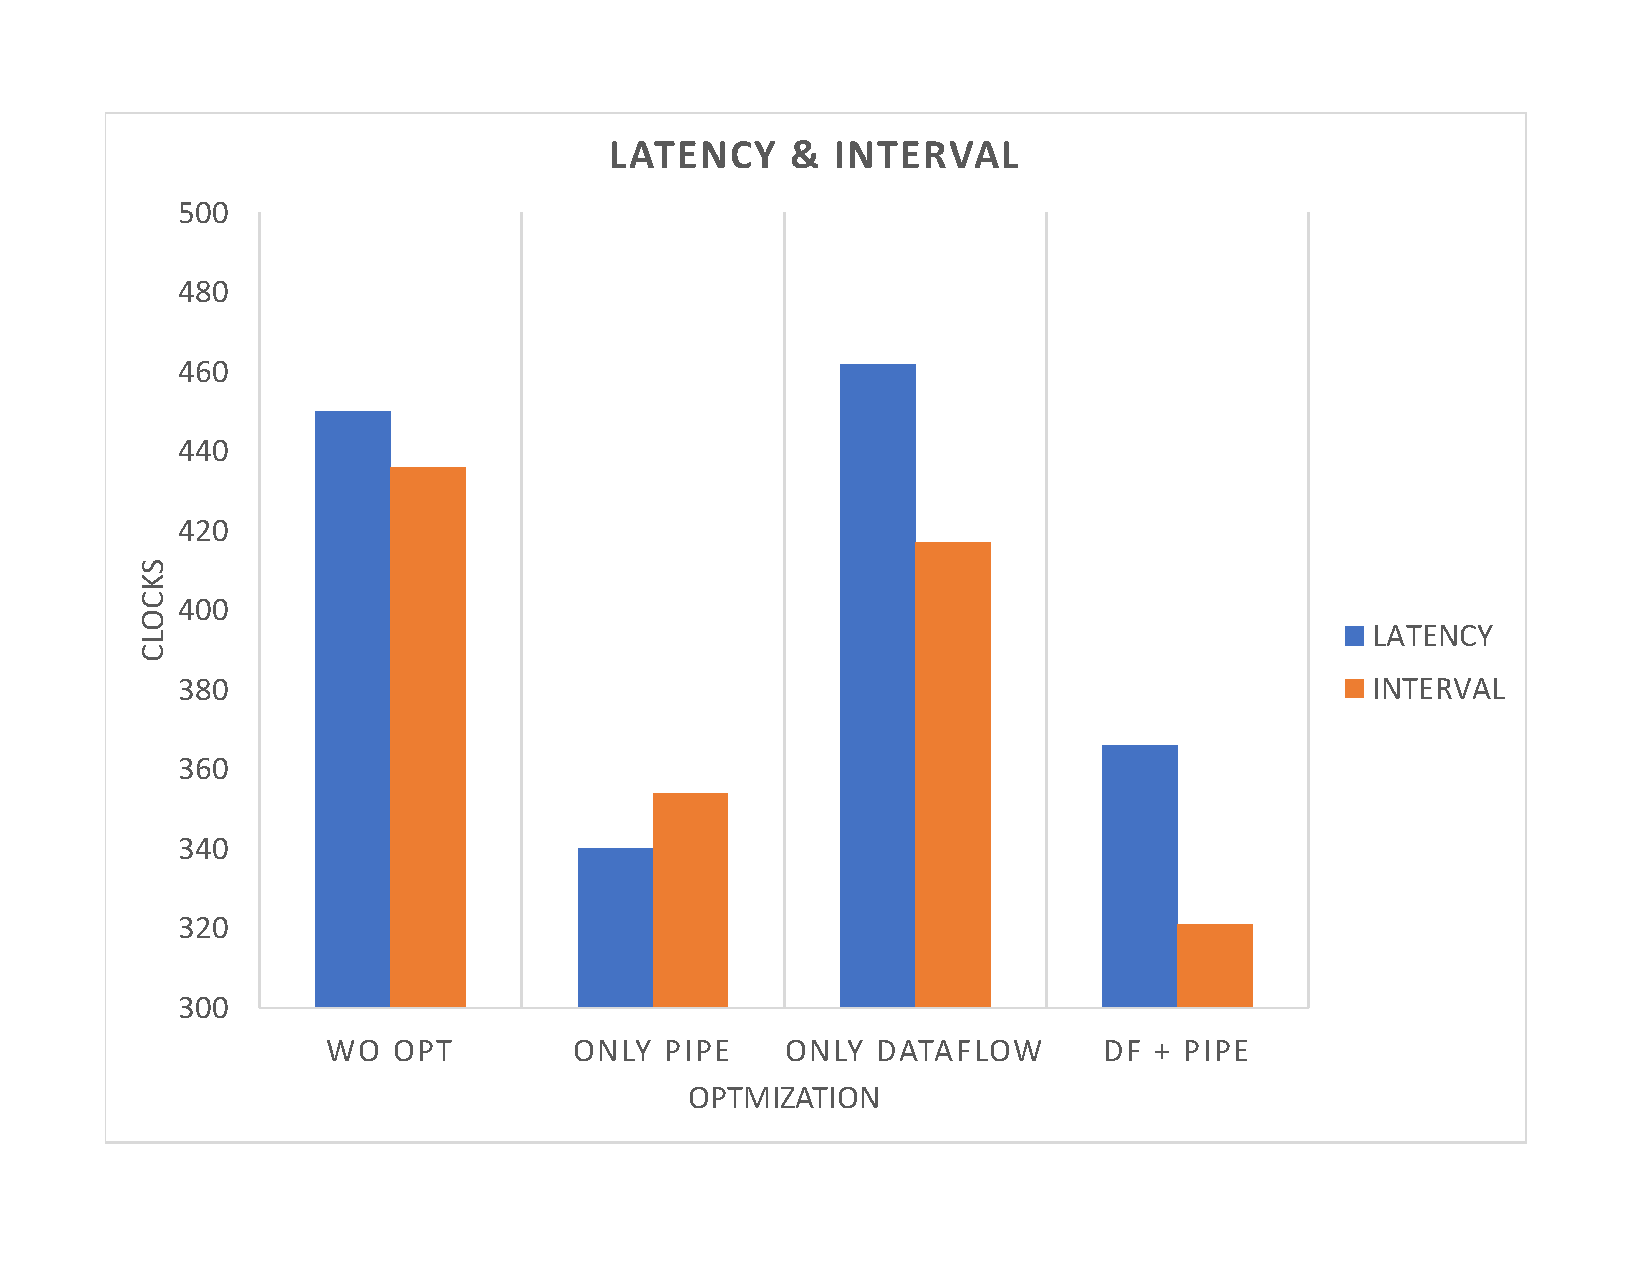
\includegraphics[scale=0.45]{Figures/LATINTFLOAT}
	\caption{Latencia e intervalo de las optimizaciones en float}
	\label{fig:latIntFloat}
\end{figure}

La Figura \ref{fig:perfGainFloat} muestra la ganancia de cada una de las optimizaciones contra la referencia (Sin optimizaciones), lo cual indica que para punto flotante, es mejor aplicar PIPELINE, obteniendo así una  reducción casi del 30\% de latencia total del circuito y 20\% más intervalo.

%tek Mirar bien los datos numéricos

\begin{figure}[!ht]
	\centering
		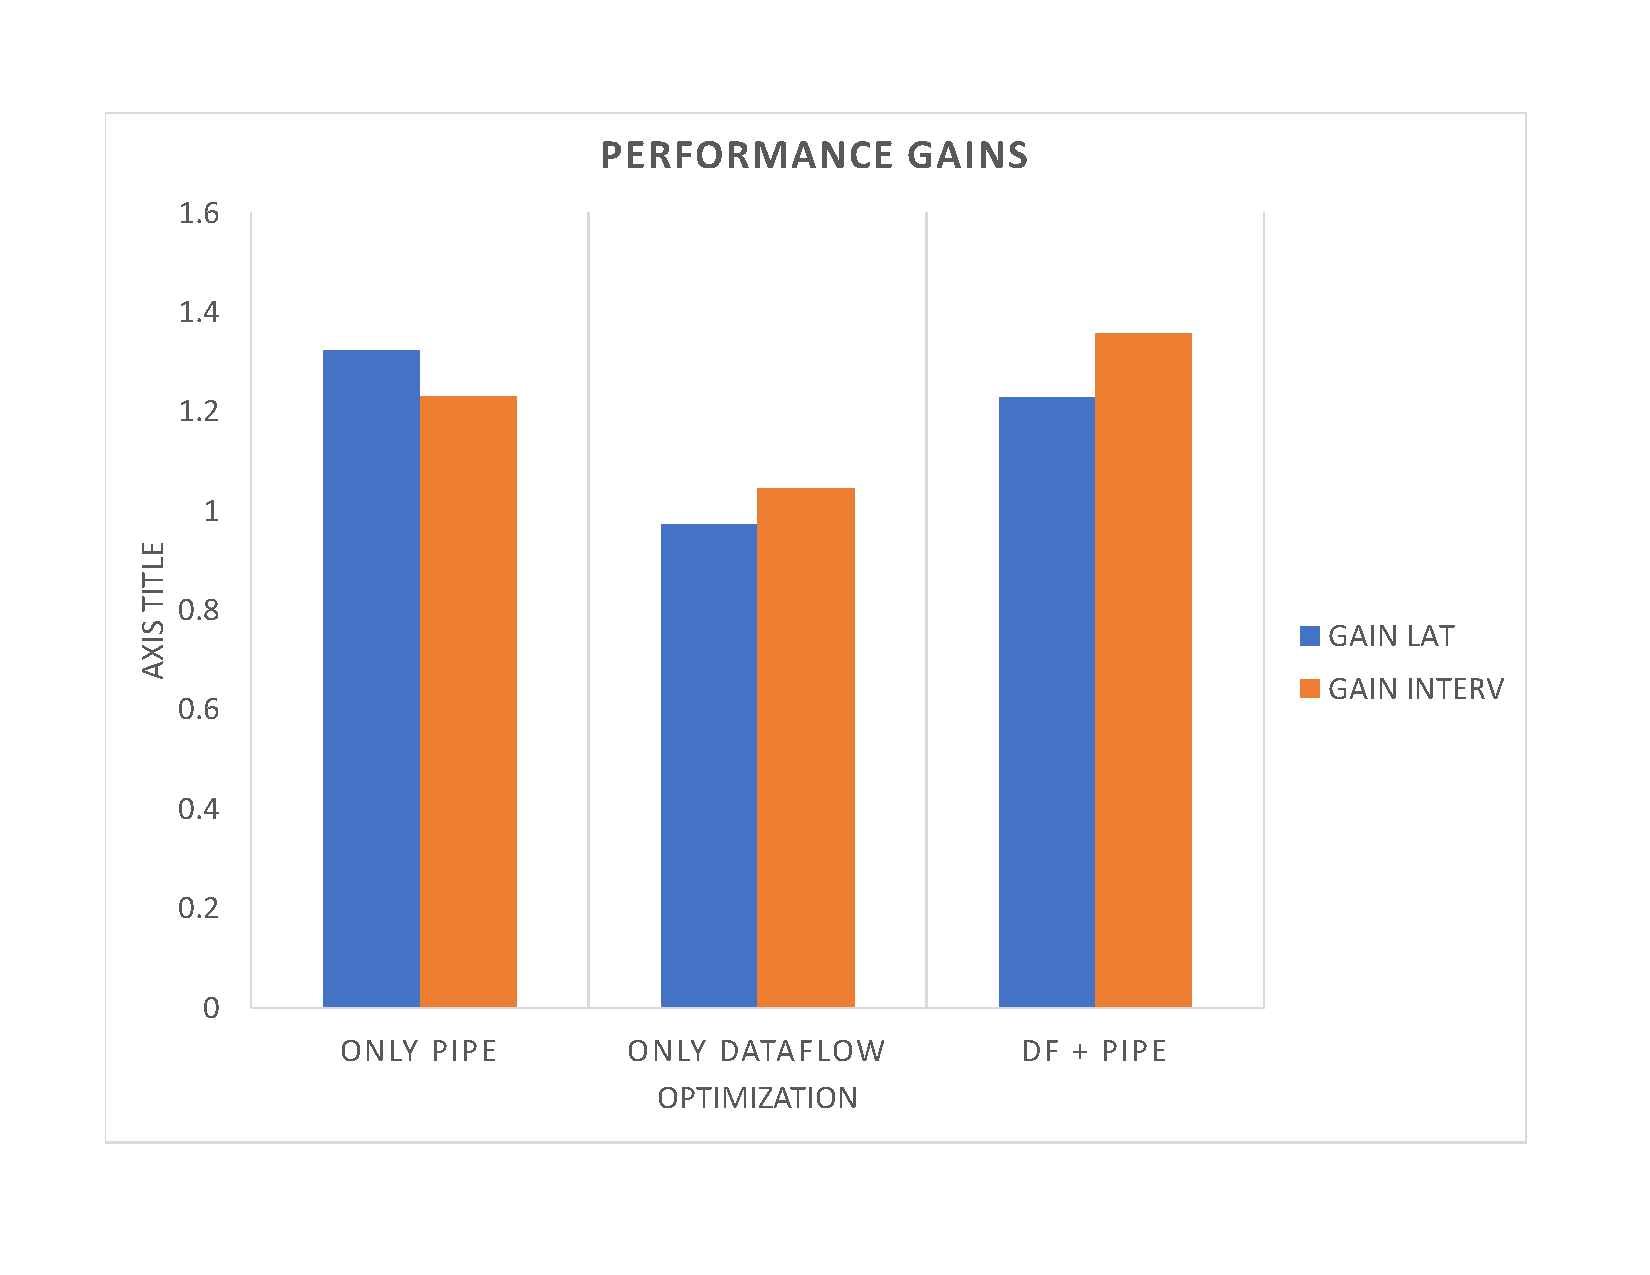
\includegraphics[scale=0.45]{Figures/PERFGAINFLOAT}
	\caption{Ganancia en rendimiento usando float}
	\label{fig:perfGainFloat}
\end{figure}

La Figura \ref{fig:latIntFix} muestra los resultados de síntesis para las mismas optimizaciones usando punto fijo.

\begin{figure}[!ht]
	\centering
		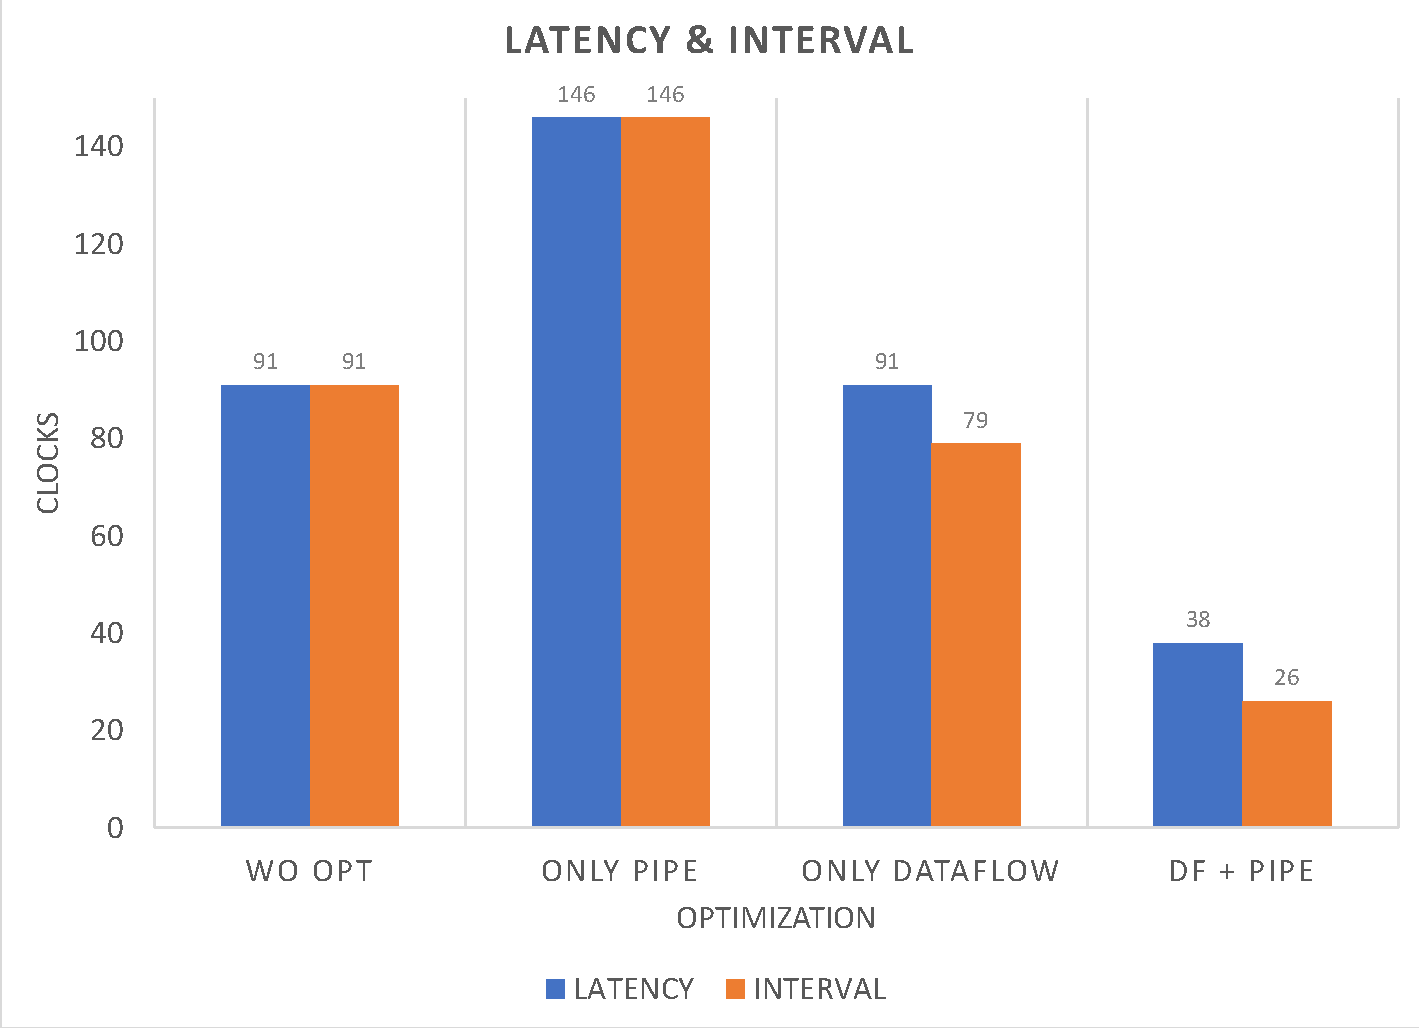
\includegraphics[scale=0.45]{Figures/LATINTFIX}
	\caption{Latencia e intervalo de las optimizaciones fijo}
	\label{fig:latIntFix}
\end{figure}

En este caso se observa un claro ganador; este puede ser corroborado por la Figura \ref{fig:perfGainFix} con 3.5 veces en mejora del intervalo y 2.5 veces de la latencia frente a la referencia.

\begin{figure}[!ht]
	\centering
		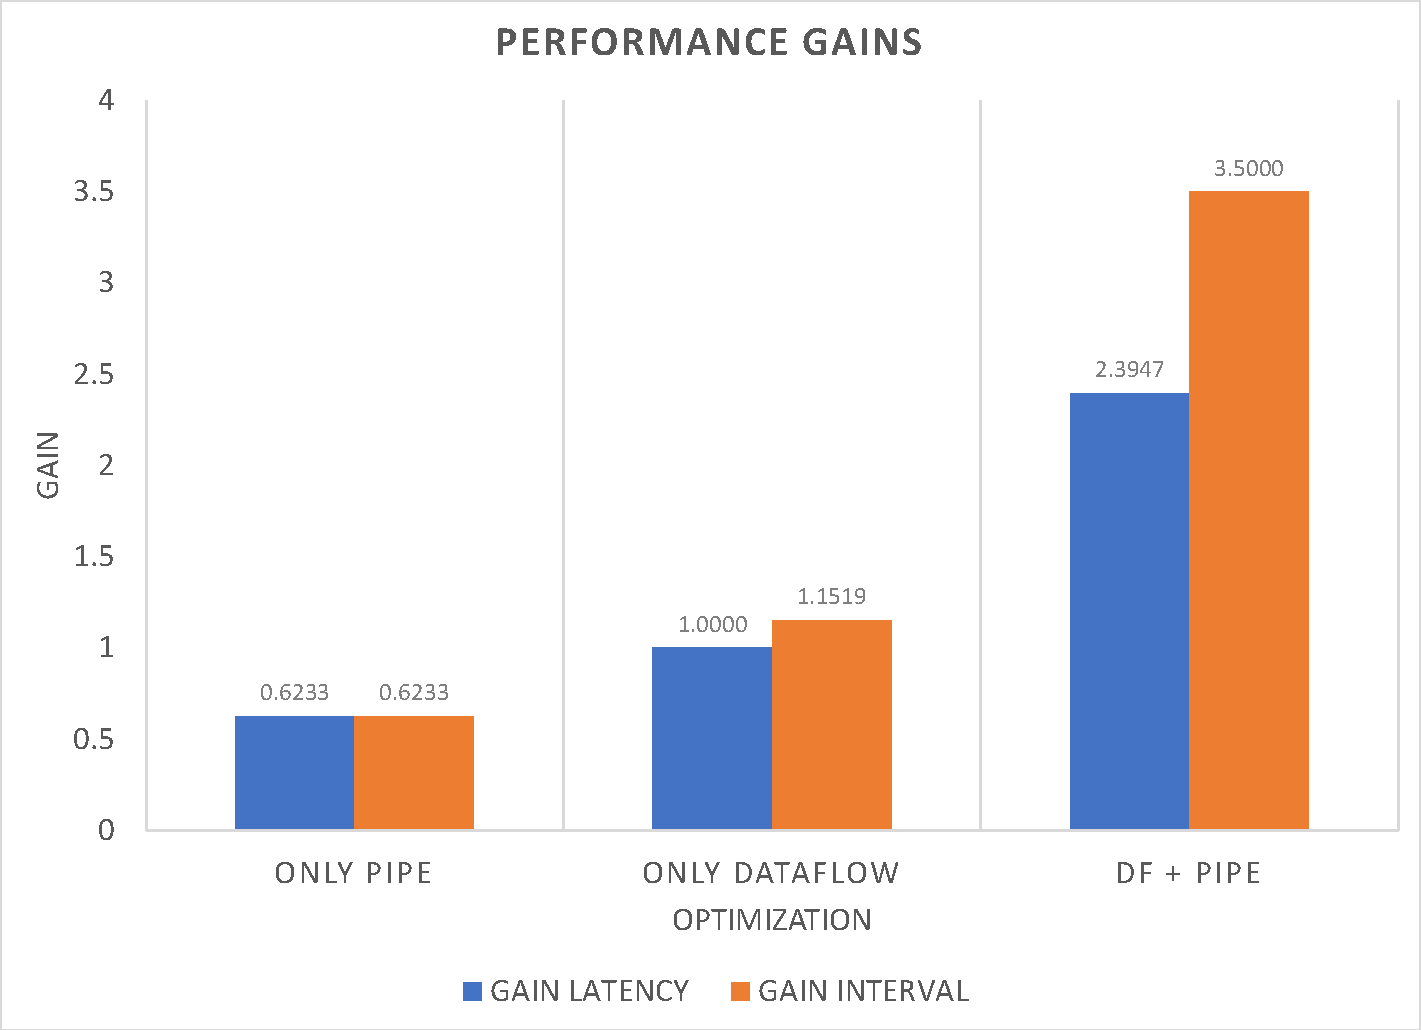
\includegraphics[scale=0.45]{Figures/PERFGAINFIX}
	\caption{Ganancia en rendimiento en float}
	\label{fig:perfGainFix}
\end{figure}

La Figura \ref{fig:fixfloat} muestra las diferencias de ganancia entre punto fijo y flotante. Es claro que las operaciones en punto fijo son menos costosas en términos de hardware; por tanto, el punto fijo y la combinación de DATAFLOW y PIPELINE son la combinación de optimizaciones a sintetizar e implementar en hardware.

\begin{figure}[!ht]
	\centering
		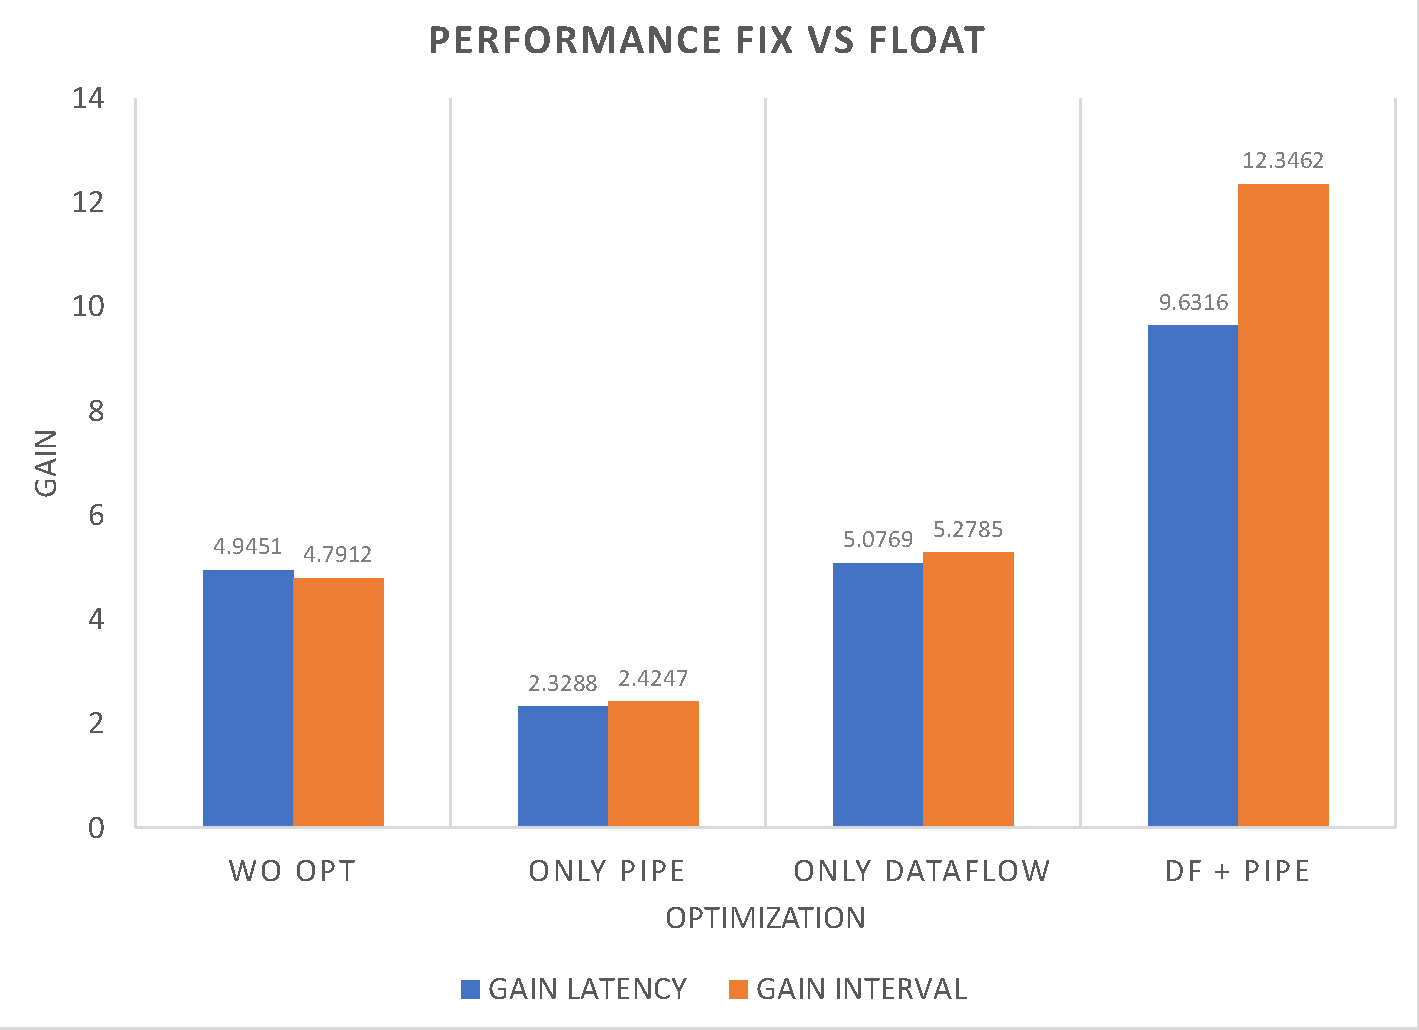
\includegraphics[scale=0.45]{Figures/fixfloat}
	\caption{Diferencia entre punto fijo y flotante}
	\label{fig:fixfloat}
\end{figure}

\subsection{Implementación del hardware}

En esta sub sección se hablará de la implementación de hardware usando el sintetizador de hardware Vivado. La Figura \ref{fig:hwImp} muestra la implementación final. En ella se observan 3 conectores AXI en el módulo \textbf{TOPANN\_0}; los de la derecha representan los maestros AXI HP, encargados de iniciar las transacciones de datos desde y hacia la memoria RAM con sus respectivos Bursts; el conector AXI Lite a la izquierda del módulo corresponde al esclavo encargado de recibir los datos de los pesos desde la memoria RAM. Se determinó que era la mejor implementación, dado que los AXI HP otorgan un ancho de banda más amplio en tanto que los pesos de la red que no cambian en el tiempo, se pueden trabajar con un puerto AXI Lite.

\begin{figure}[!ht]
	\centering
		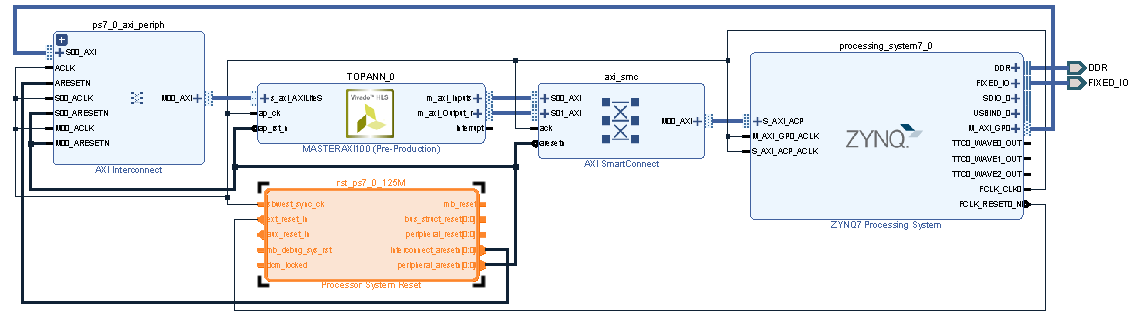
\includegraphics[scale=0.95]{Figures/hwImp}
	\caption{Implementación final de hardware}
	\label{fig:hwImp}
\end{figure} 

La Tabla \ref{tab:resourcesPostSynt} enseña la cantidad de recursos de la FPGA usados por la implementación propuesta una vez ha sido sintetizado el hardware necesario. En ella, se muestra en porcentaje usado del hardware disponible de la tarjeta de desarrollo el consumo de cada una de las unidades lógicas y de procesamiento de la FPGA por cada una de las optimizaciones propuestas. Se observa que la implementación de \textbf{DATAFLOW} más \textbf{PIPELINE} escogida para ser implementada es la que presenta mayor uso de recursos. Esto se debe al alto nivel de concurrencia que ocurre a nivel de las tareas y los buclues, otorgando un paralelismo máximo. Las implementaciones de \textbf{DATAFLOW}, \textbf{PIPE UNROLL}, y \textbf{NO OPT} son similares en cuanto a uso de hardware y su diferencia debería ser notable en tiempo de ejecución. Finalmente, en búsqueda de un equilibrio entre los recursos y el rendimiento del bloque, se configuró el sintetizador en modo de optimización de área; esto lo que garantiza es que se reutilicen los recursos de hardware disponibles de tal modo que se use la menor cantidad para implementar el circuito. En este escenario, se observa que la síntesis con optimización de área otorga una reducción de aproximadamente el 50\% en promedio de los recursos totales utilizados frente a la solución numéricamente más deseable.

%tek Revisar redacción

\begin{table}[h!]
\centering
\begin{tabular}{|c|c|c|c|c|c|c|}
\hline
 & LUT\% & \begin{tabular}[c]{@{}c@{}}LUT\\ RAM\% \end{tabular} & FF\% & BRAM\% & DSP\% & AVERAGE\% \\ \hline
\begin{tabular}[c]{@{}c@{}}DF PIPE\\ AREA OPT\end{tabular} & 27 & 12 & 15 & 13 & 15 & 16.4 \\ \hline
\begin{tabular}[c]{@{}c@{}}DF \\ PIPE\end{tabular} & 53 & 22 & 25 & 35 & 35 & 34 \\ \hline
\begin{tabular}[c]{@{}c@{}}DATA\\ FLOW\end{tabular} & 38 & 24 & 19 & 13 & 15 & 21.8 \\ \hline
\begin{tabular}[c]{@{}c@{}}PIPE\\ UNROLL\end{tabular} & 38 & 23 & 21 & 15 & 20 & 23.4 \\ \hline
\begin{tabular}[c]{@{}c@{}}NO\\ OPT\end{tabular} & 37 & 23 & 19 & 13 & 15 & 21.4 \\ \hline
\end{tabular}
\caption{Tabla uso de recursos post síntesis}
\label{tab:resourcesPostSynt}
\end{table}



%tek más óptima?

Con esto se tiene un conjunto de pruebas de cuatro circuitos diferentes para ser analizados en la plataforma de pruebas.

\section{Diseño de Software}
El diseño consta de múltiples partes. Una de ellas es el diseño de la ANN como tal; el diseño de hardware y optimizaciones a implementar; y, el esquema de reconfiguración dinámico basado en el contexto de ejecución, en este caso el estado o riesgo de inundación que pueda tener el río en un momento determinado. En esta sección se analizarán los criterios para el diseño del software; en este caso, es la capa que interconecta el hardware diseñado en la sección anterior con el procesador principal ARM A9, usando como medio el kernel de Linux.

En este caso, el diseño del software requiere conocer sobre el user space driver del kernel de Linux, que a su vez implica mapear las direcciones físicas de memoria entregadas por el módulo IP implementado en la FPGA a un espacio de memoria virtual manejado por el kernel.

La Figura \ref{fig:userSpaceDriver} muestra la mecánica de un driver funcionando bajo un esquema de espacio de usuario: el dispositivo hardware, en este caso ``Device'', recibe y escribe la información que necesita bajo una dirección física de memoria. El usuario, para acceder a esas direcciones de memoria, debe conocer la dirección base física a la cual el dispositivo está accediendo, el cual es provisto por el diseñador del hardware o en este caso el sintetizador HLS y el tamaño de paginación de memoria que entrega el SO. Con esto, el driver puede mapear la dirección de memoria a una virtual a la cual la aplicación pueda acceder como una referencia de memoria; en el caso de C/C++, como un apuntador que puede ser manipulado según sea necesario.

\begin{figure}[!ht]
	\centering
		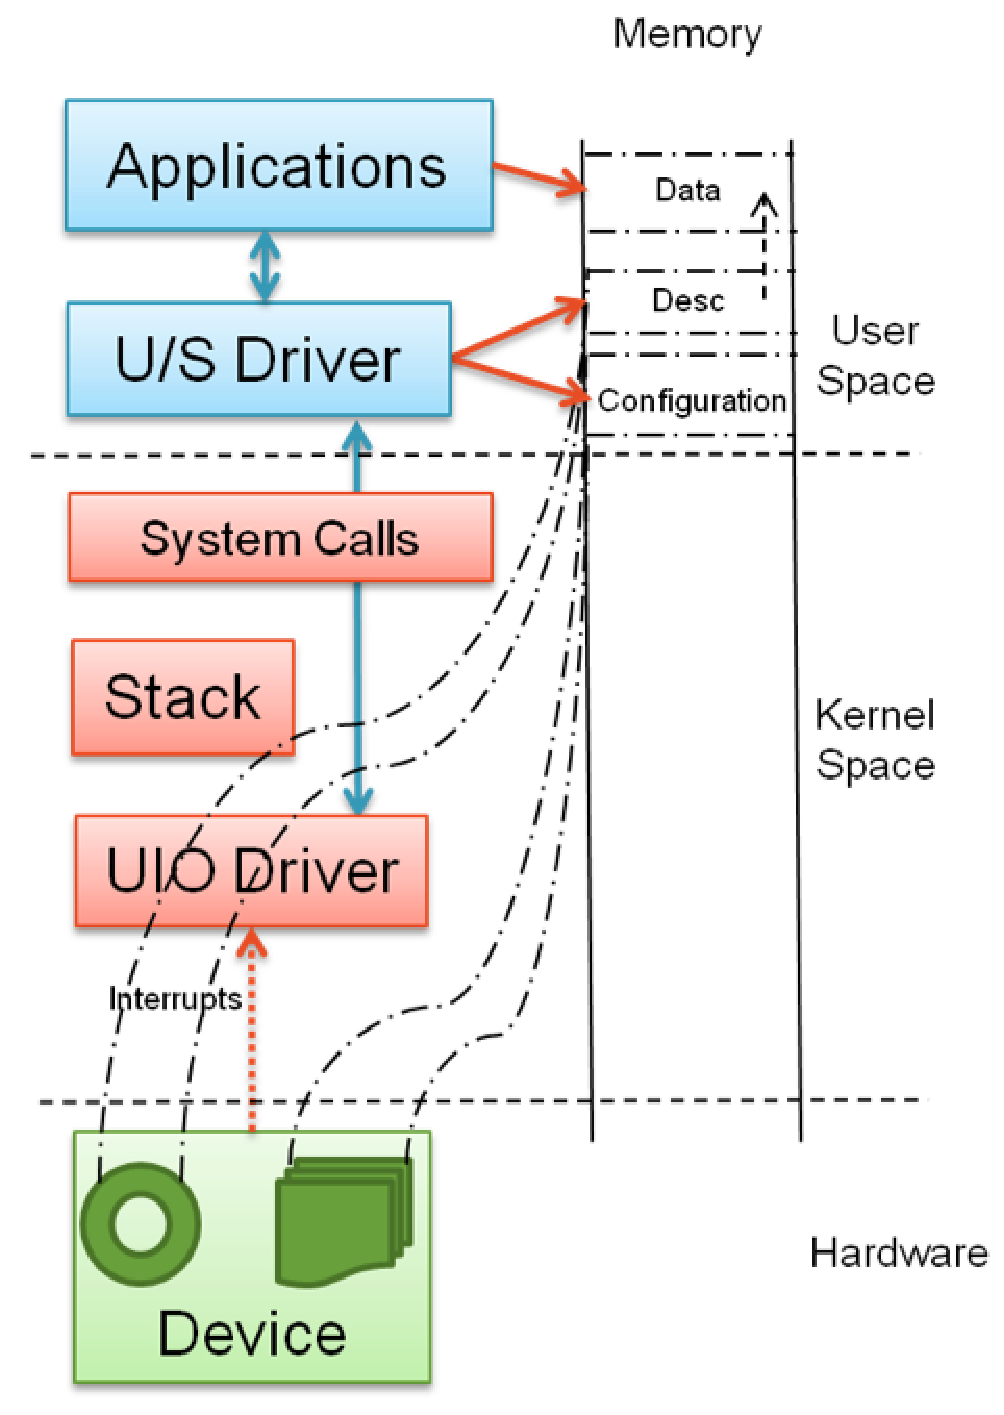
\includegraphics[scale=0.5]{Figures/UserSpaceDriver}
	\caption{Esquema de driver en espacio de usuario\cite{userSpaceDriver}.}
	\label{fig:userSpaceDriver}
\end{figure}

\subsection{Petalinux SDK}

Petalinux es una distribución especial del proyecto Yocto \citep{Yocto}, cuya razón de existir es ayudar a los desarrolladores a crear sus propias distribuciones del kernel de Linux para dispositivos embebidos. Xilinx desarrolló su propia versión del kernel basado en Yocto llamándolo Petalinux y su conjunto de herramientas conocidas como Petalinux SDK. Petalinux SDK cuenta con un gran conjunto de herramientas de compilación y ayudas al desarrollador para simplificar el proceso de personalizar y compilar el kernel de Linux para ser distribuido dentro de una de las tarjetas de desarrollo de Xilinx.

Para que un bloque IP funcione dentro de un chip ZYNQ de Xilinx debe cumplir varios requisitos.

\begin{itemize}
\item La FPGA debe ser configurada por el JTAG o por el PS7.
\item Los registros de memoria y del procesador deben ser fijados usando el procedimiento estándar de arranque descrito en la Figura \ref{fig:arranqueFPGA}.
\item Si se requiere una implementación con el kernel Petalinux, se debe garantizar que el kernel sea compilado usando Petalinux SDK con el DeviceTree y el Board Support Package (bitstream incluido) creado usando la herramienta de síntesis Vivado.
\item Se debe inicializar el bloque IP usando los registros otorgados por la herramienta de síntesis de alto nivel Vivado HLS.
\end{itemize}

\begin{figure}[H]
	\centering
		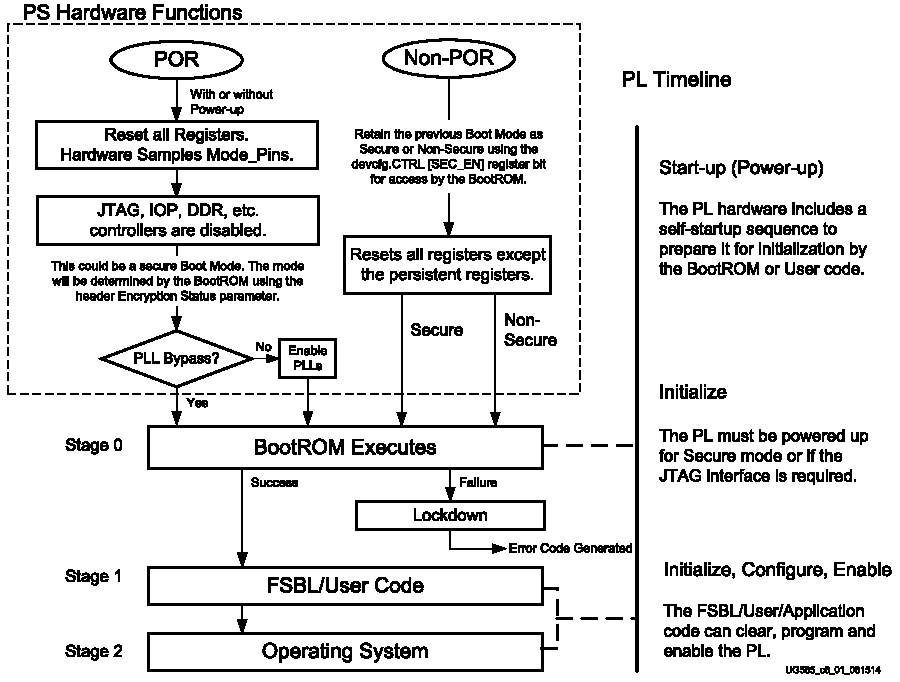
\includegraphics[scale=0.8]{./Figures/I3.pdf}
	\caption{Estructura de arranque de sistemas ZYNQ \citep{TRM2017}}
	\label{fig:arranqueFPGA}
\end{figure}

\subsubsection{Configuración de Petalinux SDK}

Dado el volumen de datos y la posibilidad de cambiar el software en línea sin recompilar el kernel de Linux se decidió que la solución debería contar con las siguientes características:

\begin{itemize}
\item Persistencia de los datos.
\item Conexión de red Ethernet.
\item Conexión serial a 115200 baudios.
\item Ejecutar software usando el User Space de Linux.
\end{itemize}

Para cumplir con lo anterior, se configura el kernel de Linux de la siguiente forma:

\begin{verbatim}
// usando bash de Linux
petalinux-config
// Una vez en el menú configurar de la siguiente manera
Image Package Configuration -> Root File System Type -> SD Card
// Salvar los cambios y salir del menú

// Usando bash de Linux
petalinux-config -c kernel
//Configurar de la siguiente manera
Device Drivers -> 
<*>User I/O platform driver with generiq IRQ handling
<*>User Platform Driver with generiq irq and dynamic memory
// Salvar y salir del menú
\end{verbatim}

Se debe garantizar la configuración del Device Tree Blob de la siguiente manera:

\begin{verbatim}
// Válido para Petalinux SDK 2017.4 y compatibles
// Modificar el archivo system-user.dtsi
// Ubicación: ./carpeta-proyecto/projec-spec/meta-user/recipes-bsp/device-tree/files

/include/ "system-conf.dtsi"
/ {

	chosen {
		bootargs = "console=ttyPS0,115200 earlyprintk uio_pdrv_genirq.of_id=generic-uio
        root=/dev/mmcblk0p2 rw rootwait";
	};

};

&TOPANN_0  {
			compatible = "generic-uio";
			reg = <0x43c00000 0x10000>;
			xlnx,s-axi-axilites-addr-width = <0x8>;
			xlnx,s-axi-axilites-data-width = <0x20>;
		};

&gem0 {
	phy-handle = <&ethernet_phy>;
/*	phy-reset-gpio = <&axi_gpio_eth 0 0>;
	phy-reset-active-low;	
	phy-reset-duration = <10>; */
	ethernet_phy: ethernet-phy@1 { /* rtl8211e-vl */
		reg = <1>;
		device_type = "ethernet-phy";
	};
};
\end{verbatim}

De esta forma, con las configuraciones dadas anteriormente, es posible compilar el kernel de Linux y con el driver adecuado debería ser posible que el hardware funcione dentro de la FPGA y sea controlado desde Petalinux.

\subsection{Diseño del driver}
Para el driver se tomó la decisión de usar el lenguaje C++ dado que permite el uso del paradigma de programación orientada a objetos, el cual permite crear diferentes módulos con funcionalidad determinada que luego pueden ser heredados a otros objetos para mejorar o ampliar el funcionamiento de los mismos. En este caso, se usaron diferentes clases u objetos que permitirían al desarrollador mapear la memoria, inicializar el módulo de aceleración de hardware con las secuencias de bits requeridos por la interfaz AXI y la operación del módulo de como tal, es decir la carga de los pesos de la ANN, los datos a procesar y los resultados de la operación.

%tek Revisar redacción

La implementación del driver se ve en la Figura \ref{fig:userSpaceDriverModel}. En ella se resumieron los métodos usados para mapear la memoria y manipular los datos que llegan y van hacia el módulo acelerador en la FPGA. La clase \texttt{ANNService} recibe como dependencia las direcciones de memoria mapeadas en la clase \texttt{Driver} mediante la clase \texttt{Controller}. La clase \texttt{ANNService} a su vez, usa la clase \texttt{ANN\_DAO}, que recibe como dependencia, una estructura de almacenamiento desacoplando la aplicación del método de persistencia. En este caso, dado que se busca obtener el performance de la aplicación como tal, se usó persistencia en memoria.

\begin{figure}[!ht]
	\centering
		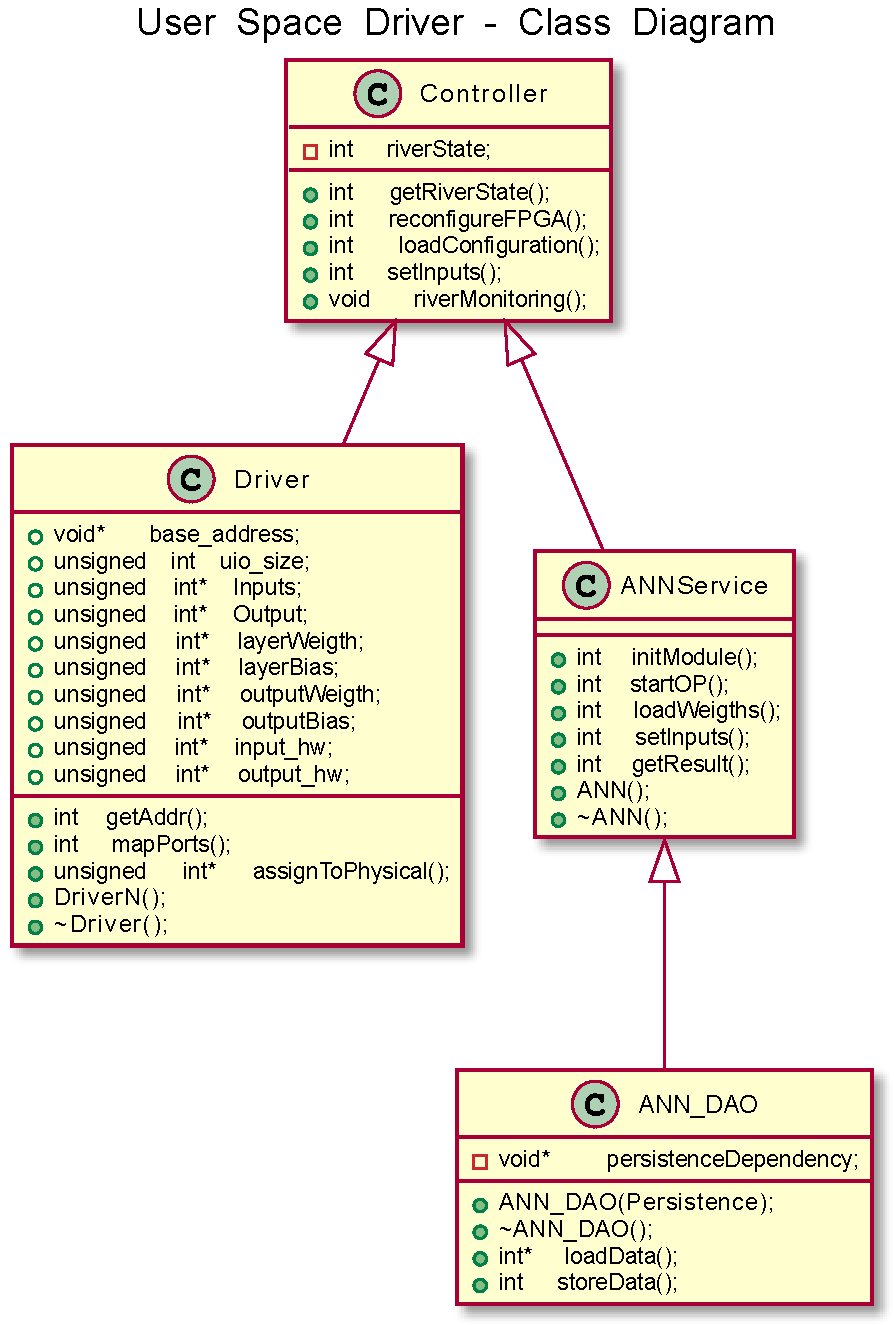
\includegraphics[scale=0.8]{Figures/driverANN}
	\caption{Diagrama de clases de la aplicación}
	\label{fig:userSpaceDriverModel}
\end{figure}

\subsection{Diseño del controlador de reconfiguración}

Teniendo en cuenta que se requiere que el controlador monitoree el estado del río mediante el estado de la ANN, se optó por un diseño reactivo del controlador, donde el riesgo de inundación disparado por la ANN activa los mecanismos de reconfiguración, la velocidad de muestreo y la recepción de datos proveniente de los nodos aledaños.

La Figura \ref{fig:esquemaFuncionamiento} muestra cómo estaría configurada la FPGA en su modo lazy o flojo, pudiendo atender los datos provenientes de los nodos aledaños cuando el Controlador detecta un riesgo de inundación; es decir que, la salida de la red ``ANN 1'' sobrepasa el umbral de entre 70\% y 80\%. Cuando el PS detecta una salida de la ``ANN 1'' sobre ese umbral, el procesador reconfigura automáticamente la FPGA para recibir un mayor número de entradas provenientes de campo. Dado que es el mismo circuito, todos estos datos pasarían por la misma interfaz AXI High Performance.

\begin{figure}[!ht]
	\centering
		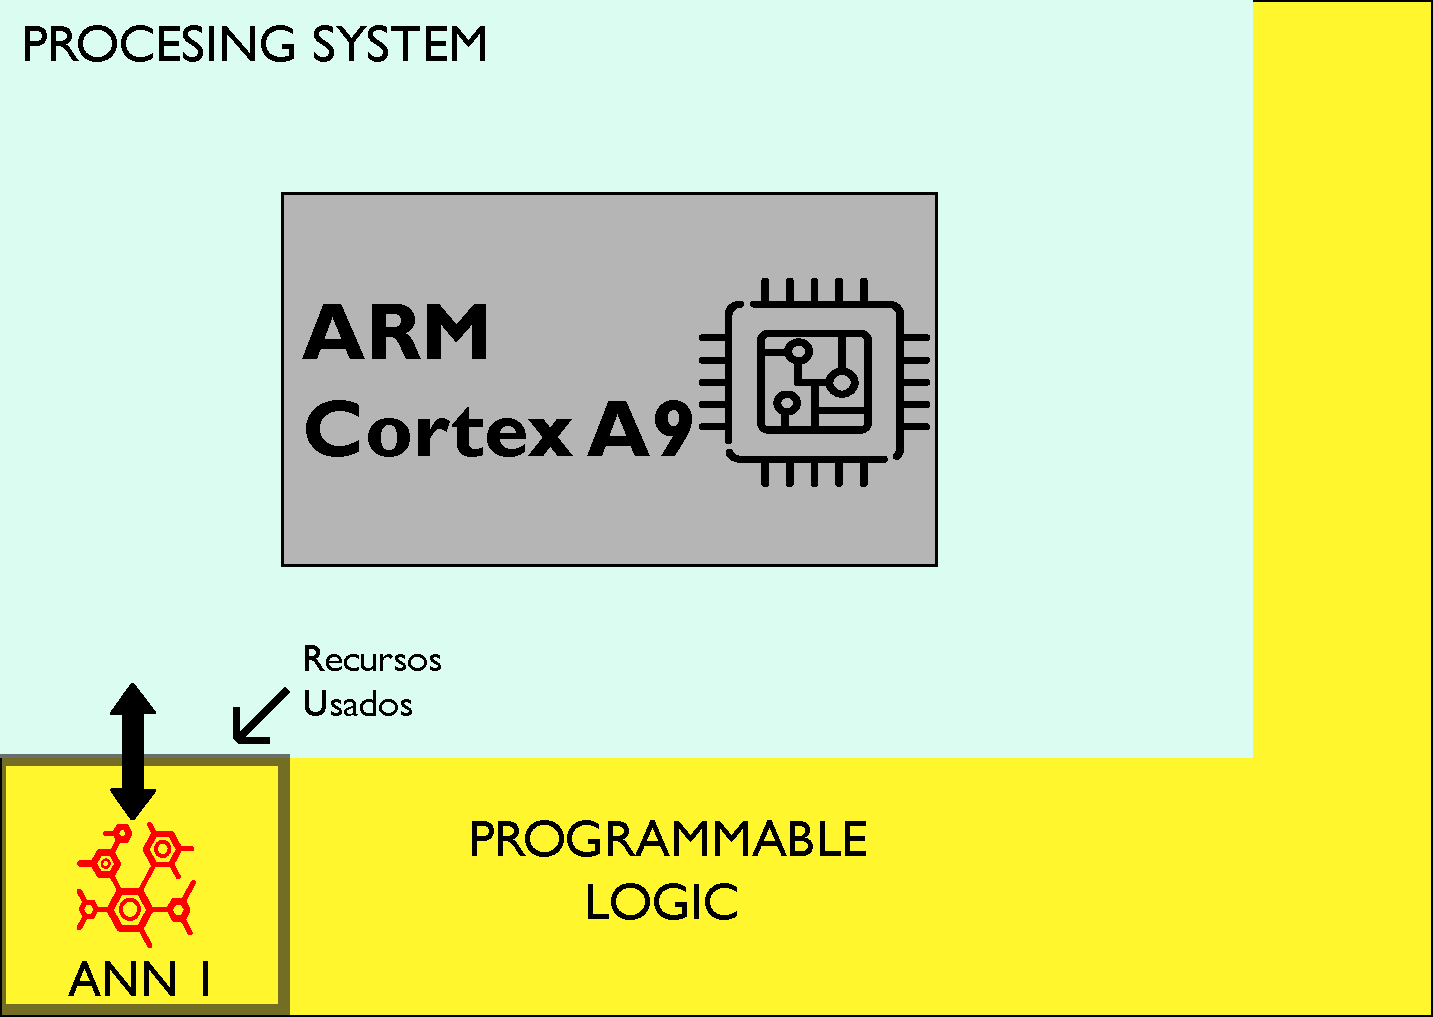
\includegraphics[scale=0.5]{Figures/ANN1}
	\caption{Esquema de funcionamiento ANN}
	\label{fig:esquemaFuncionamiento}
\end{figure}

Al reconfigurar el circuito se espera que la cantidad de área asignada al circuito cambie. En este caso, la variación está dada en función de las entradas a analizar (Neuronas de Entrada), pues se incrementa la cantidad de Look Up Tables y Block RAMs necesarias para operar la ANN.

Esto aplica también para configuraciones o aplicaciones en las que dinámicamente se adiciona hardware; la diferencia con la Figura \ref{fig:esquemaFuncionamientoReconfig}, es que se crean y se usan nuevas interfaces AXI HP que se unen al bus AMBA.

\begin{figure}[!ht]
	\centering
		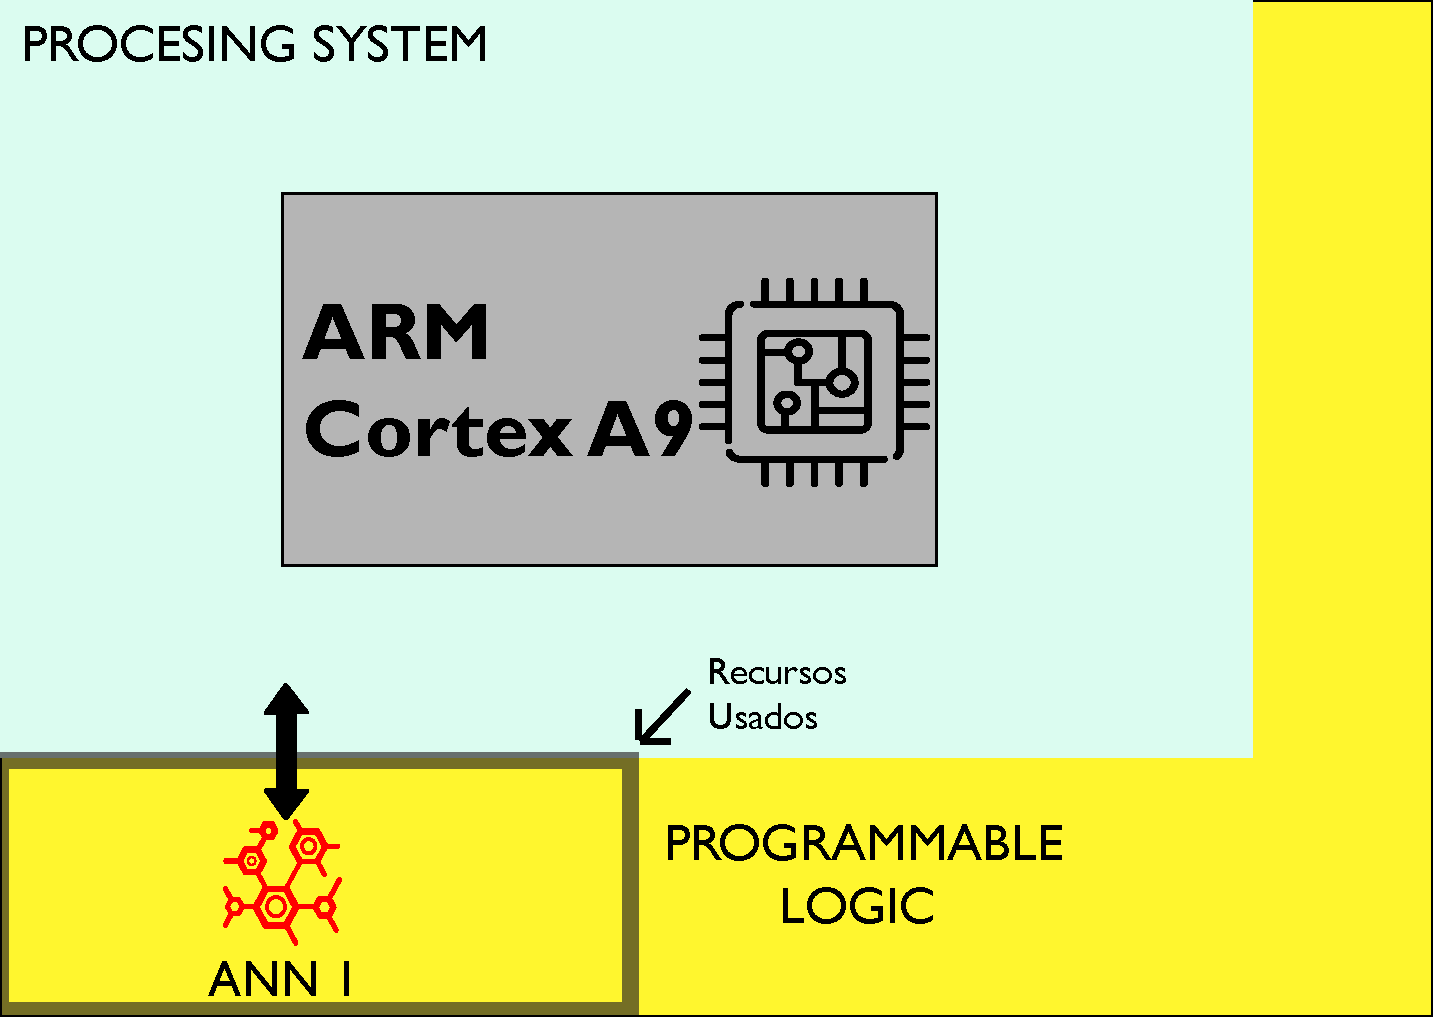
\includegraphics[scale=0.5]{Figures/ANN2}
	\caption{Esquema de funcionamiento ANN reconfigurada}
	\label{fig:esquemaFuncionamientoReconfig}
\end{figure}

La Figura \ref{fig:esquemaFuncionamientoReconfig2} muestra un esquema de configuración para múltiples aplicaciones ejecutándose en la FPGA de forma concurrente. Cada una de las instancias de las aplicaciones posee su propia interfaz AXI otorgando acceso directo a la RAM, por lo que cada una podría realizar actividades diferentes y la única actividad que debería realizar el controlador es alimentar y monitorear as direcciones de memoria correspondientes a cada uno de los bloques.

\begin{figure}[!ht]
	\centering
		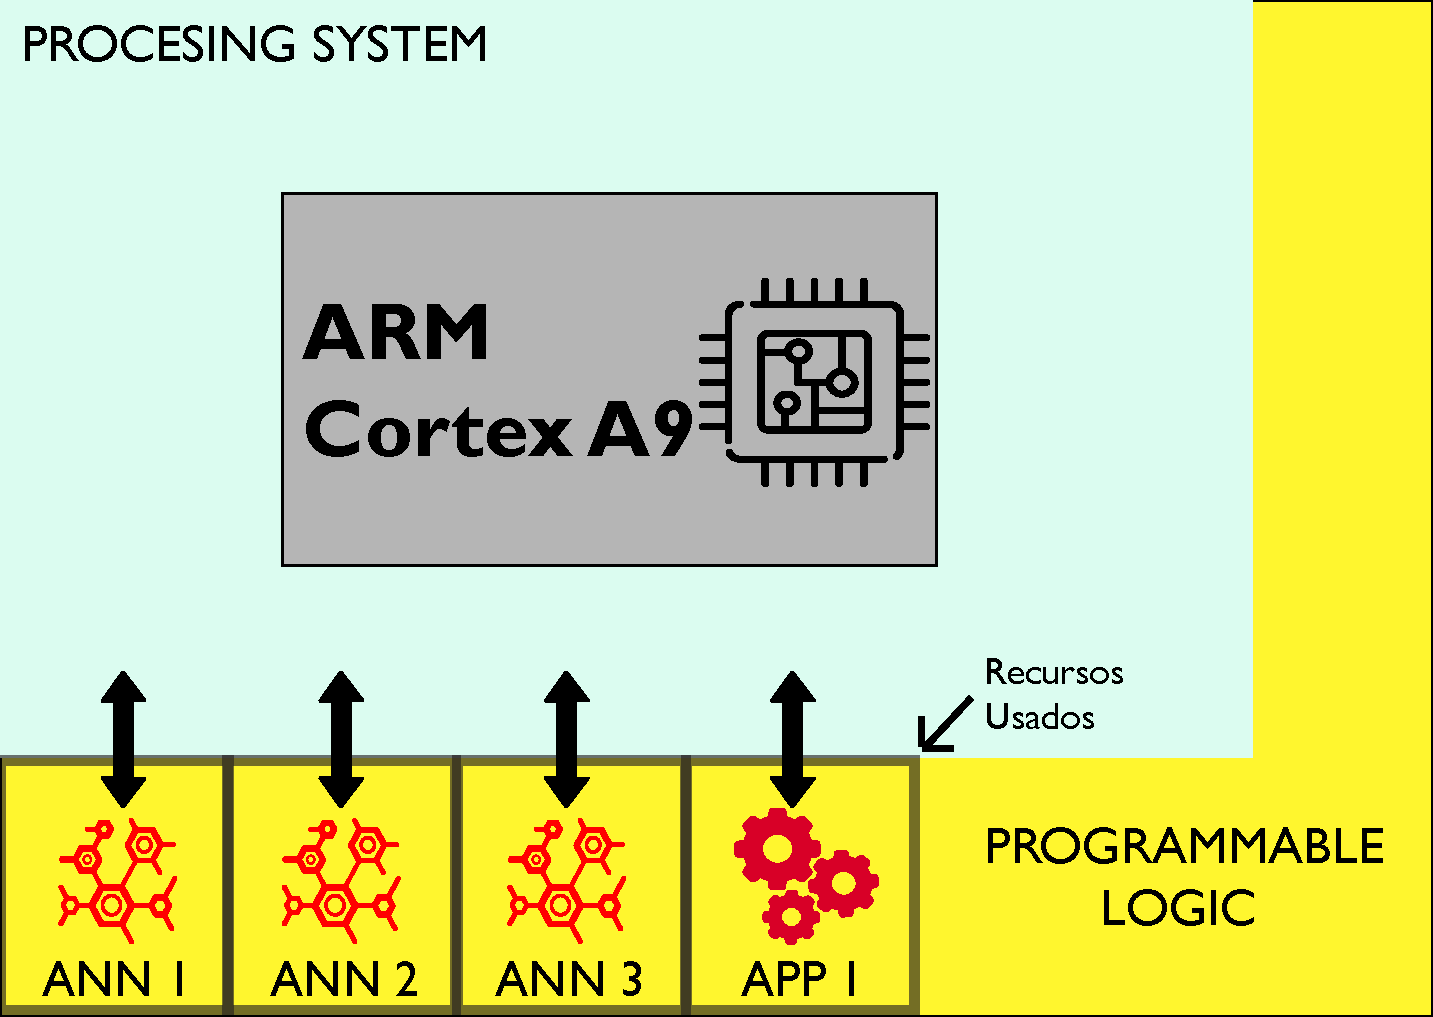
\includegraphics[scale=0.5]{Figures/ANN3}
	\caption{Esquema de funcionamiento múltiples aplicaciones}
	\label{fig:esquemaFuncionamientoReconfig2}
\end{figure}
